\documentclass[tikz,border=0pt]{standalone}
\usetikzlibrary{arrows.meta,decorations.pathmorphing,decorations.markings}

% Color settings shared across all artwork: edit palette.tex
% Edit colors HERE.  Six-digit HTML hex values, without the # character.
% This file is shared by both TikZ drawings and the build script.
\definecolor{BackgroundColor}{HTML}{000000}      % solid square background
\definecolor{ElectronColor}{HTML}{FFFFFF}        % electron propagators
\definecolor{PhotonColor}{HTML}{FFFFFF}          % wavy photon lines
\definecolor{ArrowColor}{HTML}{FFFFFF}           % electron arrows
\definecolor{VertexColor}{HTML}{FFFFFF}          % interaction vertices
\definecolor{ElectronLabelColor}{HTML}{FFFFFF}   % e labels on full diagram
\definecolor{PhotonLabelColor}{HTML}{FFFFFF}     % gamma labels on full diagram
\definecolor{SafariPinColor}{HTML}{3477C6}       % pinned-tab tint (not part of mask SVG)


% ============================================================
% DRAWING STYLES: optional adjustments
% ============================================================
\newcommand{\DiagramSize}{6}        % square side length in cm
\newcommand{\StrokeWidth}{3.6pt}    % electron / photon line thickness
\newcommand{\WaveAmplitude}{1.3mm} % height of photon wiggles
\newcommand{\WavePeriod}{5.5mm}    % length of photon wiggles
\newcommand{\VertexRadius}{0.055}  % interaction dot radius in cm
\newcommand{\LabelFont}{\fontsize{25}{28}\selectfont}
\newcommand{\LabelScale}{1.25} % adjust label size for tiny favicons

\tikzset{
  electron/.style={draw=ElectronColor,line width=\StrokeWidth,
                   line cap=round,line join=round},
  photon/.style={draw=PhotonColor,line width=\StrokeWidth,
                 line cap=round,decorate,
                 decoration={snake,amplitude=\WaveAmplitude,
                             segment length=\WavePeriod}},
  e-arrow/.style={postaction={decorate,decoration={markings,
      mark=at position 0.56 with {
        \arrow[draw=ArrowColor,fill=ArrowColor]
              {Stealth[length=17pt,width=12pt]}
      }}}}
}

\begin{document}
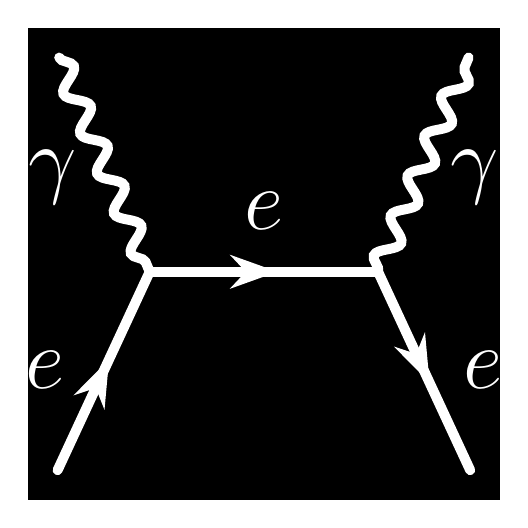
\begin{tikzpicture}[x=1cm,y=1cm]
  % Explicit square background
  \fill[BackgroundColor] (0,0) rectangle (\DiagramSize,\DiagramSize);
  \clip (0,0) rectangle (\DiagramSize,\DiagramSize); % square output

  % s-channel Compton scattering: gamma + e -> gamma + e
  \coordinate (A) at (1.55,2.90);
  \coordinate (B) at (4.45,2.90);

  % ELECTRONS: arrows point along electron flow (left -> right).
  \draw[electron,e-arrow] (0.38,0.38) -- (A);       % incoming e
  \draw[electron,e-arrow] (A) -- (B);             % virtual e (NEW arrow)
  \draw[electron,e-arrow] (B) -- (5.62,0.38);     % outgoing e

  % PHOTONS: wavy external lines
  \draw[photon] (0.40,5.62) -- (A);                % incoming gamma
  \draw[photon] (B) -- (5.60,5.62);              % outgoing gamma

  % VERTICES
  \fill[VertexColor] (A) circle[radius=\VertexRadius cm];
  \fill[VertexColor] (B) circle[radius=\VertexRadius cm];

  % ============================================================
  % FIVE PARTICLE LABELS: positions can be tweaked independently.
  % ============================================================
  \node[font=\LabelFont,scale=\LabelScale,text=ElectronLabelColor,anchor=east]
      at (0.62,1.65) {$e$};                       % incoming electron
  \node[font=\LabelFont,scale=\LabelScale,text=ElectronLabelColor,anchor=south]
      at (3.00,3.28) {$e$};                       % internal electron
  \node[font=\LabelFont,scale=\LabelScale,text=ElectronLabelColor,anchor=west]
      at (5.38,1.65) {$e$};                       % outgoing electron
  \node[font=\LabelFont,scale=\LabelScale,text=PhotonLabelColor,anchor=east]
      at (0.78,4.10) {$\gamma$};                  % incoming photon
  \node[font=\LabelFont,scale=\LabelScale,text=PhotonLabelColor,anchor=west]
      at (5.22,4.10) {$\gamma$};                  % outgoing photon
\end{tikzpicture}
\end{document}
